\documentclass[12pt]{extarticle}

\usepackage{geometry}
\usepackage{amsthm}
\usepackage{amssymb}
\usepackage{amsmath}
\usepackage{graphicx}
\usepackage{hyperref}

\graphicspath{ {./images/} }

\geometry{a4paper,
 total={170mm,257mm},
 left=20mm,
 top=20mm}

\title{Supervised Deep Learning for Optimized Trade Execution}
\author{Hua Wanying, Long Zijie, Wang Kunzhen}

\begin{document}
\maketitle

\section{Introduction}

\section{Literature Review}

\section{Model}
In this project, we assume that the optimal execution strategy can be expressed as
a pure function of the following 6 variables: $t$ the remaining time before the end of
the time horizon, $i$ the remaining inventory to sell, the price level, price trend,
limit order book volume mismatch as well as the bid-ask spread at the decision point.
Following the convention in \cite{reinforcement}, we group the 6 input variables
into two categories, i.e., the \textbf{private variables} consisting of $t$ and $i$
that is specific to the Optimized Trade Execution problem, and the \textbf{market variables}
consisting of the rest of the four. Output of the model is represented by \textit{\textbf{action}},
the price at which to place a limit order.
The model can be expressed mathematically as
$$ \textit{action} = f(t, i, \textit{price level}, \textit{price trend}, \textit{vol mismatch}, \textit{bid-ask spread}), $$
where $f$ is an unknown function to be learned. \\


\noindent To estimate the function $f$, we develop a supervised deep learning model (thereafter referred to as \textit{the model}) as described below.
The model is implemented with \textit{Tensorflow} and \textit{Tensorflow
Keras} provided by Google Brain, using \textit{Python}.
Implementation of the model can be found in the file \textit{Model.py}.\\


\begin{figure}[h]
\centering
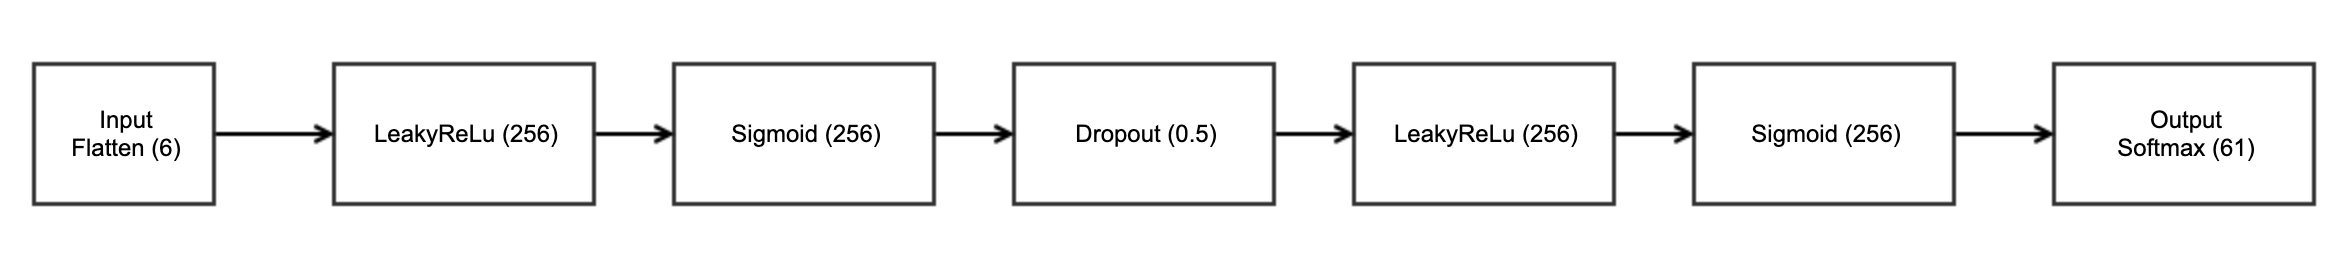
\includegraphics[width=\textwidth]{model}
\caption{The Supervised Deep Learning Model}
\end{figure}

\begin{itemize}
\item \textbf{Input Layer} The input layer consists of simply the 6 parameters of the function $f$.
Detailed definitions, rationales and extractions of these variables are
provided in Section \ref{market-variables} and \ref{private-variables}.

\item \textbf{Hidden Layers} The model is composed of 5 fully-connected hidden layers with
256 neurons each. Activation functions for each layer is, correspondingly,
\textit{leakyReLu},
\textit{sigmoid}, \textit{dropout} with a rate of 0.5,
\textit{leakyReLu}, \textit{sigmoid}. These activations are
chosen after taking into consideration the nature of the
problems. For example, noting the sparse activation characteristic of
the \textit{leakyReLu} activation and that the outputs are discrete, we chose \textit{leakyReLu}
to denoise the training process. Another advantage of the \textit{leakyReLu}
is its computational efficiency and ability to avoid dead neurons.
The \textit{sigmoid} activation is chosen for its ability to capture
non-linear relationships. A \textit{Dropout} layer is chosen
in the middle to denoise and speed up the descent. \\

\item \textbf{Output Layer} The output layer represents the predicted action given
the input. The output variable, \textit{\textbf{action}}, is discrete for computational
efficiency. Moreover, having a discretized output is important to avoid overfitting.
Refer to Section \ref{private-variables} for details on how \textit{\textbf{action}}
is discretized.

\end{itemize}


\section{Data Preparation}
This section describes in depth the dataset our research bases on and
how we extract the six aforementioned model inputs from the dataset.

\subsection{Data Description}

Describe the dataset and how we split it into training set vs testing set.

\subsection{Market Variables} \label{market-variables}

Describe the following:
\begin{itemize}
  \item How market variables are extracted from the dataset. Please include the exact formula.
  \item Rational of why those market variables are chosen.
  \item Point to the exact python file for reference.
\end{itemize}

\subsection{Private Variables} \label{private-variables}

Describe the following:
\begin{itemize}
  \item How private variables are extracted from the dataset. Please include details on
  dynamic programming (esp. formula), execution simulation, variable discretization and considerations.
  \item Point to the exact python file for reference.
\end{itemize}

\section{Model Training}
To train the model, the loss function is first determined to be the
\href{https://github.com/tensorflow/tensorflow/blob/r1.13/tensorflow/python/keras/backend.py}{\textbf{sparse categorical crossentropy}}
loss provided by \textit{Tensorflow Keras}. The loss function is one of the standard
choices in multi-categorization models, measuring the categorical crossentropy. \\


\noindent For optimization algorithm, we choose the widely used \textbf{Adam Optimizer} \cite{adam}.
It employes an adaptive learning rate and has a relatively efficient computational cost,
making use of both the first and second moments of the gradients. Key update routine
adopted by Adam is listed below.

\begin{equation*}
  \begin{split}
    g_t &\leftarrow \nabla_{\theta} f_t (\theta_{t-1}) \text{(Get gradients w.r.t. stochastic objective at time t)} \\
    m_t &\leftarrow \beta_1 \cdot m_{t-1} + (1-\beta_1) \cdot g_t \text{(Update biased first moment estimate)} \\
    v_t &\leftarrow \beta_2 \cdot v_{t-1} + (1-\beta_2) \cdot g_t^2 \text{(Update biased second moment estimate)} \\
    \hat{m_{t}} &\leftarrow \frac{m_t}{1 - \beta_1^t} \text{(Compute bias corrected first moment estimate)} \\
    \hat{v_{t}} &\leftarrow \frac{v_t}{1 - \beta_2^t} \text{(Compute bias corrected second moment estimate)} \\
    \theta_t &\leftarrow \theta_{t-1} - \alpha \cdot \frac{\hat{m_t}}{\sqrt{\hat{v_t}} + \epsilon} \text{(Update parameters)}
  \end{split}
\end{equation*}
\\


\noindent For evaluation metrics, the \href{https://github.com/tensorflow/tensorflow/blob/r1.13/tensorflow/python/ops/metrics_impl.py}{\textit{\textbf{accuracy}}}
metric provided by \textit{Tensorflow Keras} is chosen:
$$\textit{accuracy} = \frac{\textit{count}(\textit{prediction} == \textit{label})}{\textit{count}(\textit{predictions})}.$$
Ultimately it measures how often the prediction matches the label provided. \\


\noindent The model is trained with the aforementioned configurations for 2000 iterations,
at which point we note that the cost remains relatively stable and the accuracy stops
improving. Therefore, we stop the training process at 2000 iterations.

\section{Results}


\section{Remarks \& Future Work}
Despite the satisfying performance of the model, there are still plenty of room
for future improvement. We have yet to implement the improvements due to time constraint
of the project. However, we would like to note them down here as remarks.

\begin{itemize}
  \item \textbf{Loss Function} For the current model training, the metric is chosen as \textit{\textbf{accuracy}}
  to measure how often the prediction matches the label.
\end{itemize}

\section{Conclusion}


\begin{thebibliography}{9}
\bibitem{reinforcement}
Yuriy Nevmyvaka, Yi Feng, Michael Kearns.
\textit{Reinforcement Learning for Optimized Trade Execution}.
Proceedings of the 23rd International Conference on Machine Learning, Pittsburgh, PA, 2006.

\bibitem{adam}
Diederik P.Kingma, Jimmy Lei Ba.
\textit{Adam: A Method for Stochastic Optimization}.
ICLR, 2015.
\end{thebibliography}

\end{document}
